% !TEX root =  main.tex
\chapter{Introduction}
\label{chap:1}
\section{Background of Study}
\label{Sec:1.1}
\hspace{\parindent} At the microscopic scale, the physical world is in continuous, restless motion. Microscopic pollen grains or micro-scale synthetic beads suspended in still water jiggle erratically in all directions under an optical microscope. This relentless and unpredictable jiggling is known as Brownian Motion \cite{Brown1828}. First reported systematically by botanist Robert Brown in 1827 and mathematically explained by Albert Einstein in his seminal 1905 \cite{Einstein1956}, Brownian motion is driven by thermal fluctuations where millions of fast-moving solvent molecules continuously collide with larger suspended particles from all sides. When a particle experiences Brownian motion in a fluid without external guiding forces, it undergoes Pure Brownian Motion \cite{Cusi2018}. In this state, each microscopic nudge from solvent molecules is independent and unbiased. During macroscopic time intervals, these random walks cause particles to spread naturally across space through diffusion \cite{Einstein1956, Uhlenbeck1930}.

\hspace{\parindent} Diffusion plays a critical role in different fields of study such as physics, chemistry, and biology. In biological cells, key-life-sustaining processes such as enzymes locating targeted DNA strands, signaling proteins binding to receptors, or drug molecules targeting pathogens rely on diffusive searching rather than directed propulsion \cite{Redner2001,Loverdo2008}. This fundamental process introduces the Detection Problem in statistical mechanics and biological physics \cite{Benichou2011, Redner2001}. The Detection Problem evaluates the duration required for a diffusing searcher probe particle to wander through a domain and encounter a specific target foreign particle for the first time. The time required for this first collision is defined as the First-Passage Time, and its average across many search trials is the Mean First-Passage Detection Time ($\langle T\rangle$) \cite{Redner2001}.

\hspace{\parindent} In an ideal, infinitely dilute fluid, locating a target faster required deploying more searchers. If a single probe particle takes an average time $\langle T\rangle$ to detect a target,  adding identical and independent searchers ($N_p$) divides the detection time by $N_p$. This scaling rule comes from the Ergodic Theorem and the principle of Ergodicity \cite{Zwanzig2001}. In ergodic systems, observing an ensemble of $N_p$ independent searchers over a short period yields the same statistical outcome as observing a single searcher over a time period $N_p$ items longer. To measure how strictly a search system obeys this ideal behavior, the Ergodic Product ($E$) is defined as:

\begin{equation}
    E = N_p \times \langle T \rangle,
\label{eqn:1.1}
\end{equation}

\noindent In an ideal, non-interacting system, the Ergodic Product $E$ remains constant regardless of the number of probes added \cite{Loverdo2008, Zwanzig2001, Balejado2026}.

\hspace{\parindent} However, real-world physical environments are rarely dilute or non-interacting. Biological cytoplasm, microfluidic channels, and industrial colloidal suspensions are densely packed with finite-sized particles \cite{Weeks2000}. Adding probe particles to increase the search speed simultaneously increases the total Area Fraction ($\phi$) occupied by solid matter in the two-dimensional search domain. Because particles occupy physical volume and cannot overlap, increasing density toward physical packing bounds, such as the theoretical maximum Hexagonal Close Packing fraction ($\phi_{HCP} = \frac{\pi}{2\sqrt{3}}\approx 0.9069$) in two dimensions, causes excluded-volume interactions, finite collision cross sections, and steric hindrance to dominate \cite{Weeks2000,Torquato2002}. At high packing fractions, probes collide with one another and become physically trapped in temporary cages formed by their neighbors, experiencing caging dynamics or crowding \cite{Weeks2000}. Excess probe particles obstruct one another under these conditions, causing the mean detection time to rise counterintuitively and reaching a physical detection limit where adding searchers actively degrades performance \cite{Balejado2026}.

\hspace{\parindent} Understanding this trade-off between diffusion-limited search efficiency at low probe density and crowding-limited mobility suppression at high probe density requires modeling non-equilibrium mixtures containing polystyrene probe particles and smaller foreign target particles. Through particle-based Molecular Dynamics simulations using Large-scale Atomic/Molecular Massively Parallel Simulator (LAMMPS) \cite{Thompson2022} and continuous Langevin dynamics \cite{Coffey2004}, this thesis explores the onset of crowding, quantifies the breakdown of ergodicity using the Ergodic Product $E$, and determines the optimal probe density window for foreign particle detection \cite{balejado2026}.

\section{Theoretical Framework and Key concepts}
\label{sec:1.2}
\hspace{\parindent} A particle undergoing Pure Brownian Motion experiences a continuous series of uncorrelated random collisions from surrounding fluid molecules. According to the Langevin model \cite{Uhlenbeck1930, Coffey2004}, the equation of motion for a spherical particle of mass $m$ and position $r(t)$ is expressed as follows:

\begin{equation}
    m\frac{d^2r}{dt^2}=-\gamma\frac{dr}{dt}+F_{random}(t)
\label{eqn:1.2}
\end{equation}

\noindent where $\gamma = 6 \pi \eta r$ represents the Stoke drag coefficient in a fluid with dynamic viscosity $\eta$ and particle radius $r$. The term $F_{random}(t)$ is a rapidly fluctuating stochastic force with zero mean ($\langle F_{random}(t) \rangle =0$) representing Gaussian white noise. Over time intervals $\tau$ much larger than momentum relaxation time or Langevin damping parameter ($\tau_{damp} = \frac{m}{\gamma}$), the particle loses memory of its initial velocity. By the Central Limit Theorem \cite{Feller1968}, the net displacement $\Delta x = x(t+\tau) -x(t)$ resulting from the sum of independent microscopic collisions approaches a normal gaussian distribution centered at zero mean:

\begin{equation}
    P(\Delta x) = \frac{1}{\sqrt{4\pi D\tau}}exp\left(-\frac{(\Delta x)^2}{4D\tau}\right),
\label{eqn:1.3}
\end{equation}

\noindent where $D$ is the Self- Diffusion Coefficient \cite{Einstein1956}.

\hspace{\parindent} Diffusion quantifies how rapidly a particle explores space. In $d$-dimensional space, Einstein's diffusion relation connects single-particle movement to time through the Mean Squared Displacement (MSD) \cite{Einstein1956, Cusi2020}:

\begin{equation}
    \sigma^2 = \mathrm{MSD} = \overline{[(x(t+\tau)-x(t))^2]} = 2dD\tau
\label{eqn:1.4}
\end{equation}

%not sure if this should be indented or not
\noindent for two-dimensional systems ($d=2$), MSD$(\tau) = 4$D$\tau$. From an experimental or computational trajectory, the MSD Diffusion Coefficient ($D_{MSD}$) is extracted from the linear slope ($m_{slope}$) of the MSD($\tau$) versus sampling time interval ($\tau$) curve \cite{Cusi2020, balejado2025}:

\begin{equation}
    D_{MSD} = \frac{m_{slope}}{2d} = \frac{m_{slope}}{4}
\label{eqn:1.5}
\end{equation}

\noindent alternatively, leveraging the Gaussian displacement distribution dictated by the Central Limit Theorem, the Displacecment-Variance Diffusion Coefficient ($D_{var}$) is extracted by calculating the spatial variance ($\sigma_x^2, \sigma_y^2$) of displacement distrbutions across independent trajectory intervals \cite{Cusi2020, balejado2025}:

\begin{figure}[t]
    \centering 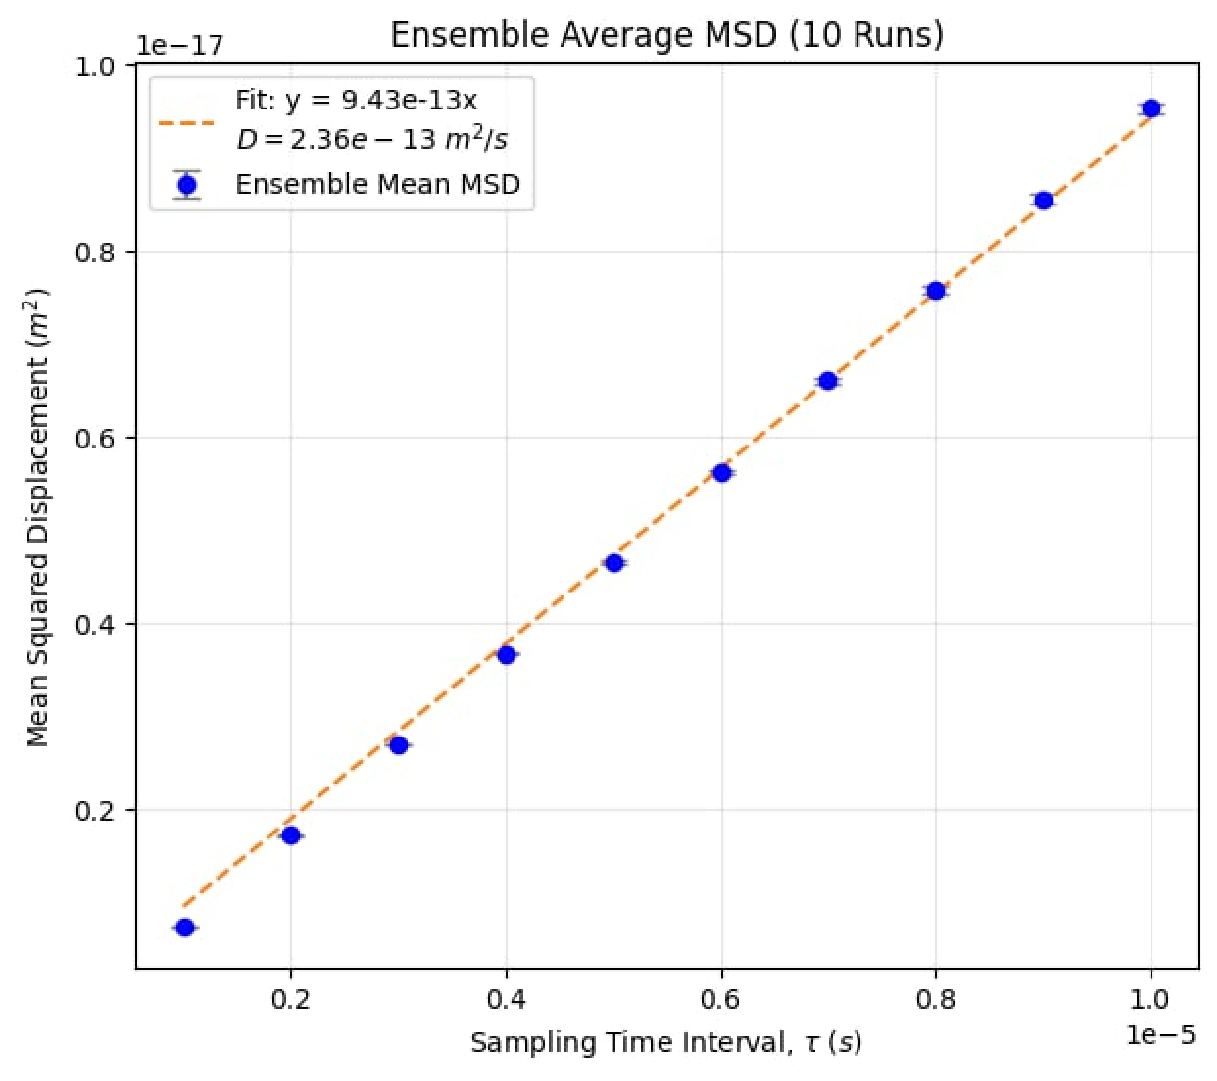
\includegraphics[width=0.48\textwidth]{figures/Probe_MSD.pdf}
    \hfill 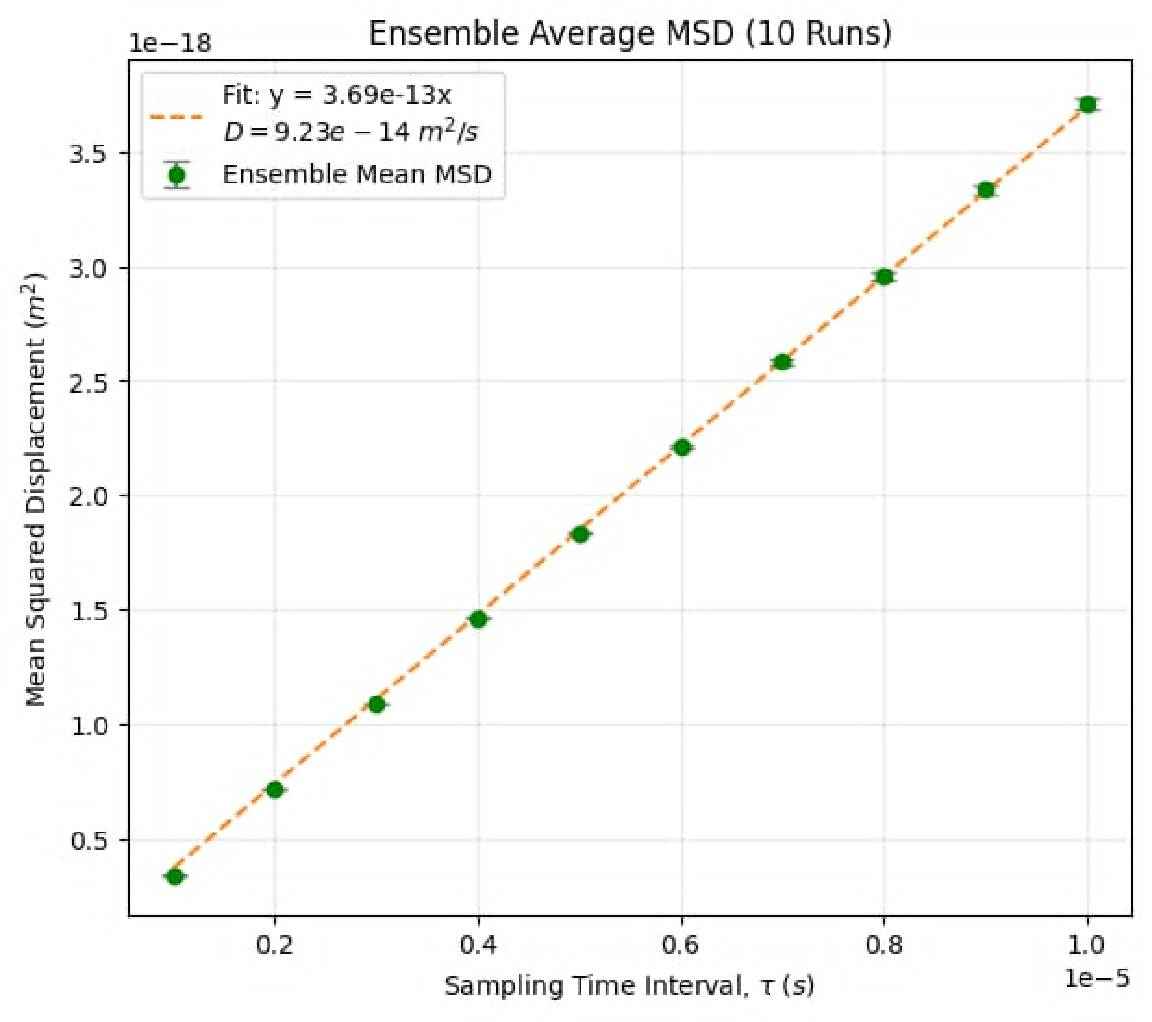
\includegraphics[width=0.48\textwidth]{figures/Foreign_MSD.pdf}
    
    \caption{Ensemble-average mean squared displacement versus sampling interval $\tau$ for the (a) probe and (b) foreign particle species, with linear fits used to extract $D_\text{MSD}$.}
    \label{fig:side_by_side_plots}
\end{figure}

\begin{equation}
    D_{var} = \frac{\sigma_x^2+ \sigma_y^2}{2d\tau} = \frac{\sigma_x^2+ \sigma_y^2}{4\tau}
\label{eqn:1.6}
\end{equation}

% To fix, I will make the plots 2x2 so it will be bigger
% \begin{figure}[b]
%     \centering
%     \subfigure{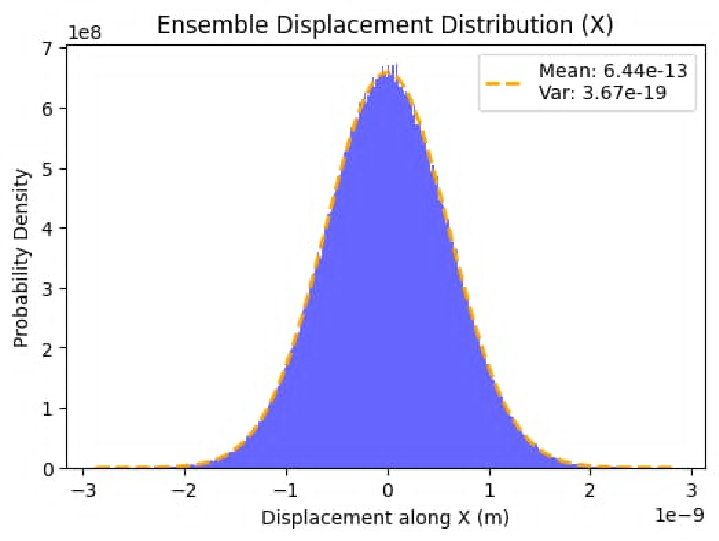
\includegraphics[width=0.25\textwidth]{figures/Probe_Disp_X.pdf}%
%     }%
%     \hfill
%     \subfigure{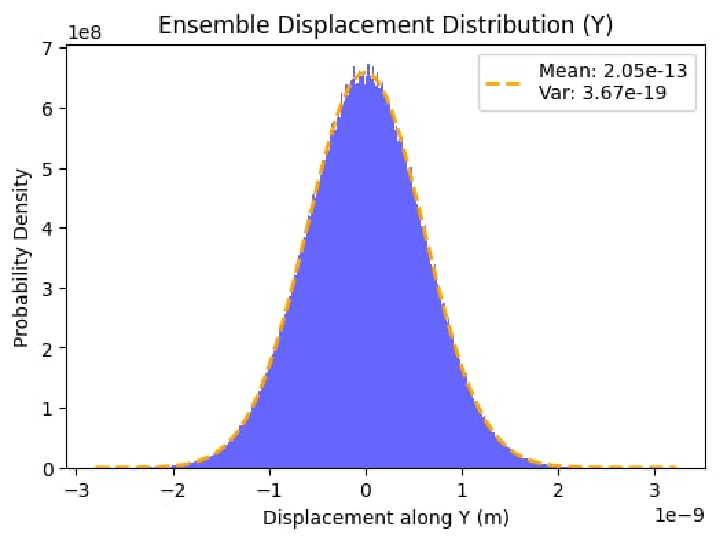
\includegraphics[width=0.25\textwidth]{figures/Probe_Disp_Y.pdf}%
%     }%
%     \hfill
%     \subfigure{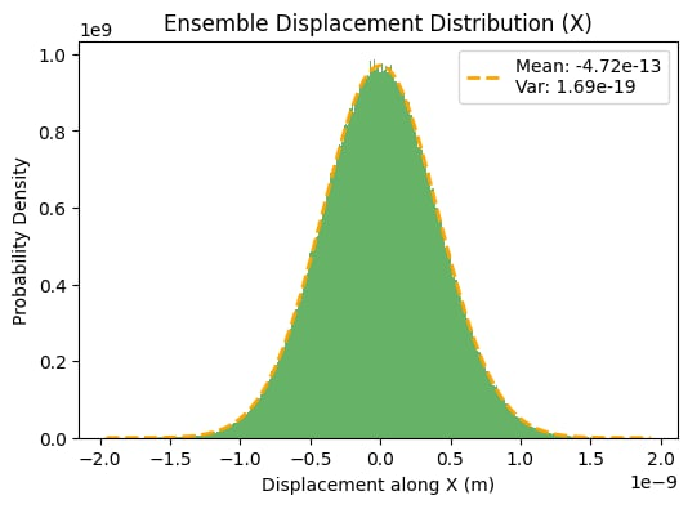
\includegraphics[width=0.25\textwidth]{figures/Foreign_Disp_X.pdf}%
%     }%
%     \hfill
%     \subfigure{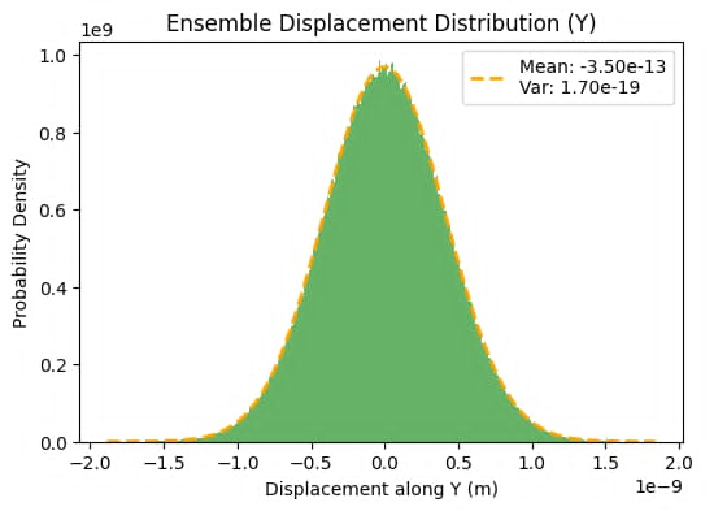
\includegraphics[width=0.25\textwidth]{figures/Foreign_Disp_Y.pdf}%
%     }%
    
%     \caption{Ensemble displacement distribution along x for the (a) probe and (b) foreign particle species, with Gaussian fits confirming the CLT-predicted profile used to extract $D_\text{var}$}
%     \label{fig:four_plots}
% \end{figure}
\begin{figure}[h]
    \centering
    % Top Row
    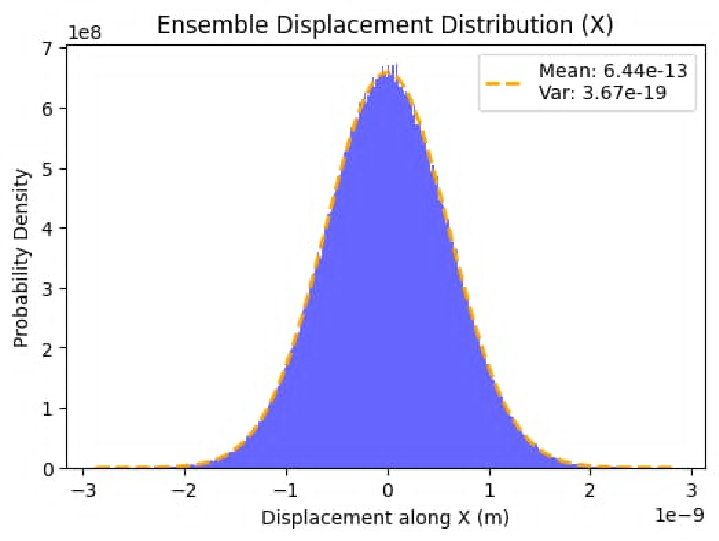
\includegraphics[width=0.48\textwidth]{figures/Probe_Disp_X.pdf}%
    \hfill
    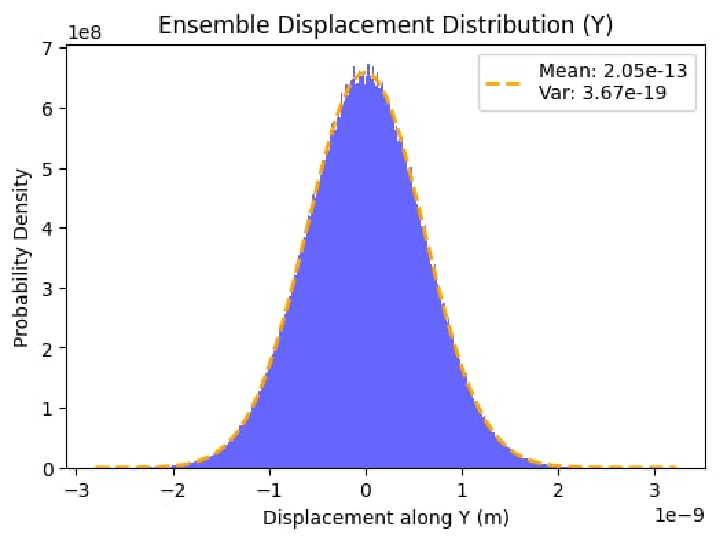
\includegraphics[width=0.48\textwidth]{figures/Probe_Disp_Y.pdf}%
    \\[0.5em] % Vertical space between top and bottom rows
    % Bottom Row
    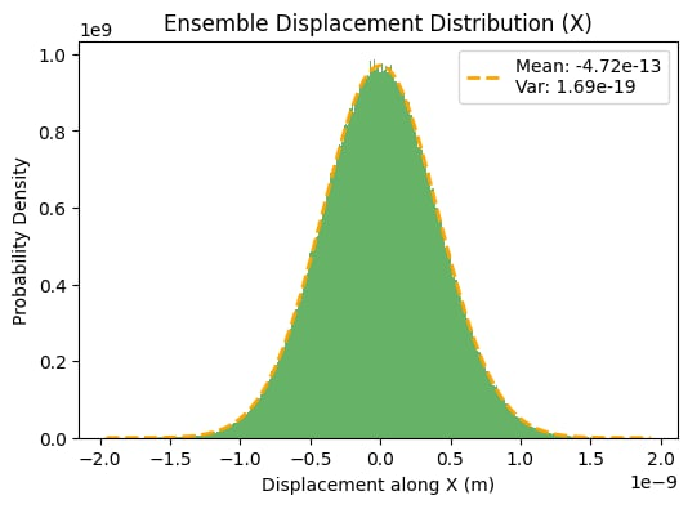
\includegraphics[width=0.48\textwidth]{figures/Foreign_Disp_X.pdf}%
    \hfill
    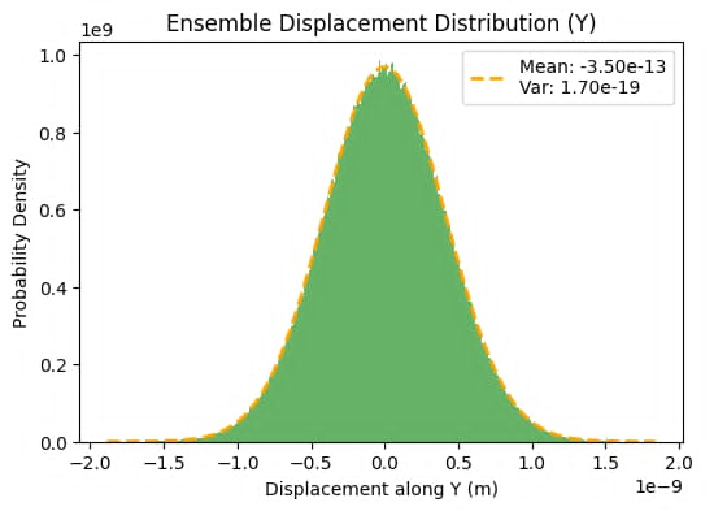
\includegraphics[width=0.48\textwidth]{figures/Foreign_Disp_Y.pdf}%
    
    \caption{Ensemble displacement distributions along $x$ and $y$ for the probe and foreign particle species, with Gaussian fits confirming the CLT-predicted profile used to extract $D_\text{var}$.}
    \label{fig:four_plots}
\end{figure}

\noindent ensuring that the sampling time $\tau$ is significantly longer than the Langevin damping parameter ($\tau >> \tau_{damp}$) is essential to avoid the deterministic ballistic motion regime ($\tau \leq \tau_{damp}$) and achieve precise agreement with the theoretical Stoke-Einstein diffusion coefficient \cite{Einstein1956, balejado2025}:

\begin{equation}
    D_T = \frac{k_BT}{6\pi\eta r},
\label{eqn:1.7}
\end{equation}

\noindent where $k_B$ is the Boltzmann constant and $T$ is absolute temperature.

\hspace{\parindent} When $N_p$ Brownian polystyrene probe particles wander inside a domain containing target foreign particles, the primary physical quantity of interest is the first-passage detection time $T$. This is defined as the time step at which any probe particle first comes within a specified interaction distance $R_{int}$ of a foreign target particle, accounting for the collision cross section $\sigma_{\alpha \beta}$ \cite{Redner2001}. When probe density is low, probes do not interfere with each other. Under the Ergodic Theorem \cite{Zwanzig2001}, the ensemble average across searchers is equivalent to the time average of a single searcher exploring space over an extended duration. Consequently, $\langle T\rangle \propto \frac{1}{N_p}$, meaning the Ergodic Product $E = N_p \times \langle T \rangle$ remains constant \cite{Loverdo2008}. When the Ergodic Product $E$ remains flat across varying probe counts, the system operates within the ergodic, diffusion-limited search regime.

\hspace{\parindent} As $N_p$ grows, the total occupied surface area increases. The system density is measured by its Area Fraction ($\phi$) \cite{Balejado2026}:

\begin{equation}
    \phi = \frac{N_p \pi r_p^2 + N_f \pi r_f^2}{A_{box}},
\label{eqn:1.8}
\end{equation}

\noindent where $N_p$ and $r_p$ are the number and radius of probe particles, $N_f$ and $r_f$ are the number and radius of foreign target particles, and $A_{box} = L \times L$ is the area of the square box subject to periodic boundary conditions. To prevent physical overlap between finite-sized particles, short-range repulsive interactions are modeled using the Weeks-Chandler-Andersen (WCA) soft repulsion potential \cite{Weeks1971}:

\begin{equation}
    U_{WCA}(r) = \begin{cases}
        4\mathcal{E}\left[\left(\frac{\sigma}{r}\right)^12-\left(\frac{\sigma}{r}\right)^6\right] + \mathcal{E}, &r\leq2^{1/6}\sigma \\
        0, & r\geq 2^{1/6}\sigma
    \end{cases},
\label{eqn:1.9}
\end{equation}

\noindent where $\varepsilon$ sets the interaction energy scale and $\sigma$ represents the effective hard-core collision diameter. As $\phi$ increases toward dense packing regimes, probes frequently collide with neighbors, causing available free space to contract and trapping particles inside temporary cages \cite{Weeks2000}. This transition marks the boundary of the crowding-limited search regime, where adding more probes increases $\langle T\rangle$ and causes $E$ to deviate upward from linearity.

\section{Statement of the Problem}
\label{sec:1.3}
\hspace{\parindent} In microscopic search and capture systems, maximizing detection speed while managing the concentration of probes is a primary practical challenge. While adding searchers accelerates detection times in open fluids, deploying excess probe particles in confined or dense environments triggers steric hindrance, reduces diffusive mobility, and increases detection times \cite{Torquato2002, Weeks2000}. Although first-passage dynamics in dilute media are well established theoretically \cite{Redner2001}, a number of key questions remain open regarding crowded, multi-sized non-equilibrium mixtures.

\hspace{\parindent} Specifically, this study addresses how varying probe density directly impacts mean first-passage detection times ($\langle T\rangle$) across different system scales ($N_{total}$). It determines the exact area fraction ($\phi$) threshold where a two-dimensional Brownian system transitions from a diffusion-limited search to a crowding-limited search. Furthermore, it investigates whether the Ergodic Product ($E = N_p \times \langle T\rangle$) can serve as an earlier, more sensitive order parameter for detecting the onset of spatial crowding compared to monitoring $\langle T \rangle$ alone, while evaluating how overall system scale modifies the physical detection limit in crowded colloidal environments \cite{Balejado2026}. As part of characterizing this transition, this thesis also proposes a fourfold qualitative typology for classifying how sharply the crowding-limited response manifests as a function of system scale with the typology consisting of Incipient, Shield, and Steep-Walled, and the Bifurcated caldera profiles.


\section{Objectives of the Study}
\label{sec:1.4}
\hspace{\parindent} The study uses two-dimensional Brownian dynamics simulations to analyze how probe density and excluded-volume crowding affect first-passage target detection efficiency. The primary objective is to construct particle-based Brownian dynamics simulations in \texttt{LAMMPS} modeling non-equilibrium mixtures of polystyrene probe particles ($d_p = 2.0\, \mu$m) and foreign target particles ($d_f = 1.0 \,\mu$m) under periodic boundary conditions \cite{Thompson2022}. Pure Brownian dynamics are verified by calculating diffusion coefficients via both Mean Squared Displacement ($D_{MSD}$) and Displacement-Variance ($D_{var}$) techniques, validating them against theoretical Stokes-Einstein predictions ($D_{th}$) \cite{Einstein1956, Cusi2020, balejado2025}.

\hspace{\parindent} Furthermore, this work quantifies the Mean First-Passage Detection Time ($\langle T \rangle$) across a wide range of probe numbers ($N_p$) and system ensemble sizes ($N_{total} = 10, 30, 50, 70, 100, 200$) across multiple independent simulation seeds. The ergodic product ($E = N_p \times \langle T \rangle$) is evaluated as a diagnostic parameter to pinpoint the exact transition from ergodic diffusion-limited dynamics to non-ergodic crowding-limited dynamics \cite{Loverdo2008}. Finally, this study identifies the optimal probe density window that maximizes foreign target detection efficiency before caging effects impair probe mobility. 

\section{Significance of the Study}
\label{sec:1.5}
\hspace{\parindent} This work provides insights across physics, biophysics, soft condensed matter, and bio-nanotechnology. Biological cells are packed with macromolecules occupying $20\,\%$ to $40\,\%$ of cellular volume \cite{Loverdo2008, Benichou2011}. This study provides a framework for understanding how crowding alters reaction rates, search strategies, and transport efficiency inside living cytoplasm \cite{Loverdo2008, Redner2001}.

\hspace{\parindent} In automated point-of-care microfluidic diagnostic devices, functionalized magnetic or polystyrene beads are introduced to detect rare pathogens or trace analytes. Determining the optimal probe density prevents fluid clogging and minimizes diagnostic detection times while reducing reagent costs. From a theoretical perspective, by testing the breakdown of the Ergodic Theorem in soft-core particle suspensions, this research contributes to the fundamental understanding of non-equilibrium statistical mechanics, glassy caging dynamics, and multi-agent stochastic search optimization \cite{Redner2001, Zwanzig2001, Weeks2000}.

\section{Scope and Limitation of the Study}
\label{sec:1.6}
\hspace{\parindent} To ensure a focused physical investigation, the parameters and computational boundaries of this study are defined carefully. Simulations are restricted to two-dimensional (2D) square spatial domains with periodic boundary conditions, mimicking thin fluid films, microfluidic chips, or biological membrane surfaces. Probes are modeled as polystyrene spheres with diameter $d_p = 2.0 \,\mu$m, while foreign target particles have diameter $d_f = 1.0\,\mu$m, maintaining a $2:1$ diameter ratio. Particle mass density is set to $\rho = 1050$ \,kg/m$^3$ in water at $T = 298\,$K ($\eta = 0.89\,$mPa$\cdot$s).

\hspace{\parindent} interparticle collisions are modeled strictly via short-range repulsive Weeks-Chandler-Andersen (WCA) potentials \cite{Weeks1971}. Long-range electrostatic charges, hydrodynamic interactions between moving spheres, and particle gravity or buoyancy effects are excluded. Computational trajectories are generated using \texttt{LAMMPS} \cite{Thompson2022}, visualized using \texttt{OVITO} (Open Visualization Tool) \cite{Stukowski2010}, and post-processed using custom \texttt{Python} analysis workflows using \texttt{NumPy}, \texttt{SciPy}, and \texttt{Matplotlib}.